%%%%%%%%%%%%%%%%%%%%



%\part{Regresión lineal simple}
%\frame{\partpage}

%\frame{
 % \frametitle{Índice}
%  \frametitle{Outline of Part I}
%\tableofcontents[pausesections,part=1]
%}

\chapter{Regresión lineal simple}

\section{Introducción}


\begin{frame}



\frametitle{Introducción}



\begin{block}{Introducción}
\uncover<2-> {Consideremos los pares de observaciones de dos variables:$$\{(x_i,y_i)| i=1,2,\ldots,n\}$$}
\begin{itemize}
\item<3-> La variable $y$ es la variable dependiente o de respuesta.

\item<4-> La variable $x$ es la variable de control o
independiente o de regresión.

\item<5-> El problema que se intenta resolver es encontrar la mejor relación
funcional que explique la variable $y$ conocido el valor de la
variable $x$:$Y/x$. En nuestro caso esta función será una recta.
\end{itemize}
\end{block}
\end{frame}

\begin{frame}



\frametitle{Ejemplo}

\begin{block}{}
\uncover<2->{Ejemplo: Consideremos los datos siguientes donde $x$ representa los meses e $y$ representa el crecimiento de un determinado tipo de planta en mm.
\vskip0.25cm
\begin{center}
\begin{tabular}{|r|r|}
\hline
Meses & Crecimiento \\
\hline\hline
12   &   0 \\\hline
10   &   1 \\\hline
8    &   2 \\\hline
11   &   3\\\hline
6    &   4\\\hline
7    &   5\\\hline
2    &   6\\\hline
3    &   7\\\hline
3    &   8\\\hline
\end{tabular}
\end{center}}
\end{block}
\end{frame}

\begin{frame}

\frametitle{Ejemplo}

\begin{block}{}
\uncover<2->{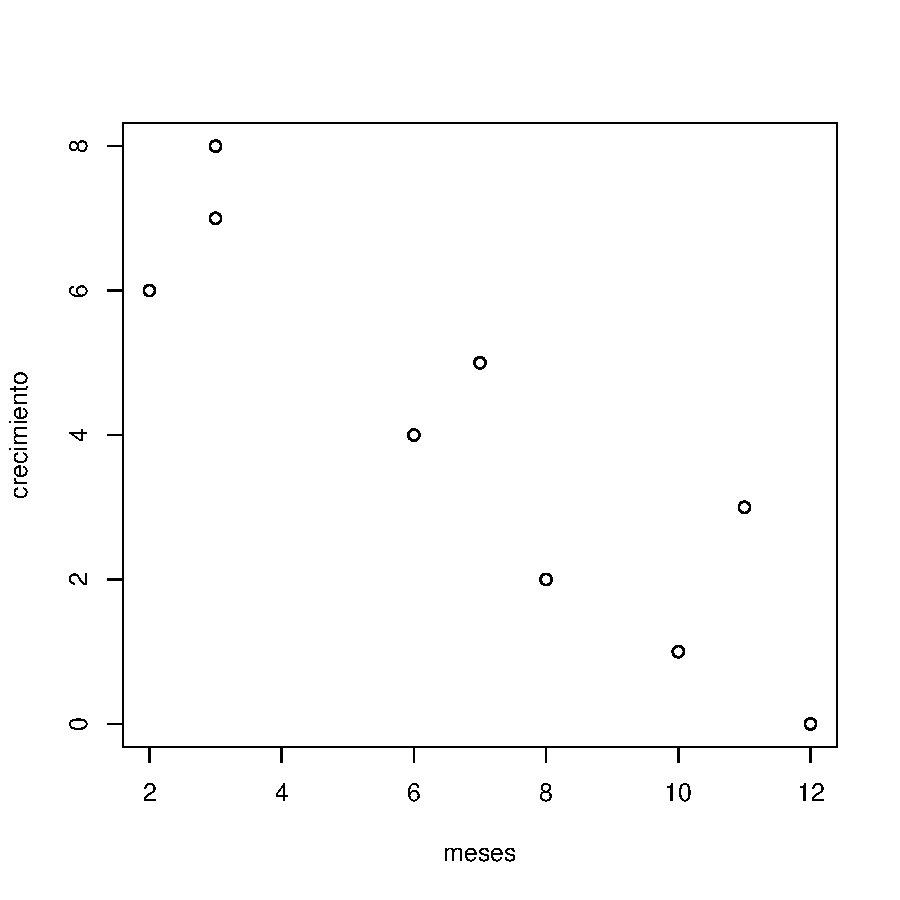
\includegraphics[scale=0.5]{GrapRLS.pdf}}
\end{block}


\end{frame}


\section{El modelo}
\begin{frame}
\frametitle{El modelo de Regresión lineal simple}
\begin{block}{}
\uncover<2->{En realidad, en un análisis más riguroso, el modelo de regresión
lineal es el siguiente:
$$\mu_{Y/x}=\beta_0+\beta_1 x,$$
donde $\mu_{Y/x}$ es el valor esperado  que toma la variable $y$
cuando la variable de control vale $x$, mientras que $\beta_0$
(término independiente) y $\beta_1$ (pendiente) son dos
parámetros a determinar.
}
\end{block}
\begin{block}{}
\uncover<3->{Dada una muestra calcularemos las estimaciones $b_0$ y $b_1$ de
$\beta_0$ y de $\beta_1$ respectivamente. Notemos que para
muestras diferentes, las estimaciones serán diferentes.

Una vez obtenidas las estimaciones podemos calcular la recta de
regresión estimada, que es:\newline
$\hat{y}=b_0+b_1 x.$}
\end{block}

\end{frame}

\section{Mínimos cuadrados}
\begin{frame}
\frametitle{Regresión lineal simple por Mínimos cuadrados}

\begin{block}{}
\begin{itemize}
\item<2->{Existen diversas maneras de calcular las estimaciones de  los
coeficientes de una regresión lineal: Regresión ortogonal, métodos
robustos, regresión mínimo cuadrática o de mínimos cuadrados,...
Nosotros optaremos por el método más habitual que es el de mínimos
cuadrados (m.c.).}
\item<3->{Modelo
$$Y_i=\beta_0+\beta_1 x_i+ E_i,$$
Donde $E_i$ es una nueva variable llamada error o residuo.}
\item<4->{Una vez planteado el modelo  y dada una muestra el modelo se debe
ajustar a los datos de ésta:
$$y_i=\beta_0+\beta_1 x_i+ E_i,\, \mbox{para } i=1,2,\ldots n.$$}
\end{itemize}
\end{block}
\end{frame}

\begin{frame}
\frametitle{Regresión lineal simple por Mínimos cuadrados}

\begin{itemize}
\item<2->{Cuando ajustamos por las estimaciones $b_0$ y $b_1$
obtenemos la recta de regresión ajustada
$$\hat{y}=b_0+b_1 x.$$}

\item<3->{Podemos calcular para cada par de observaciones:

$$y_i= b_0+b_1 x_i+e_i,\qquad \hat{y_i}=b_0+b_1 x_i \mbox{ para } i=1,2,\ldots n.$$}
\item<4->{Entonces el error o residuo de la $i$-ésima observación,
$i=1,2,\ldots,n$, es
$$e_i=y_i-\hat{y}_i.$$}
\end{itemize}
\end{frame}

\subsection{Cálculo de los coeficientes}
\begin{frame}
\frametitle{Regresión lineal simple por Mínimos cuadrados}

\framesubtitle{Cálculo de los coeficientes}

\begin{block}{Cálculo de $b_0$ y $b_1$ por M.C.}
\begin{itemize}
\item<2->{Los valores de $b_0$ y $b_1$ buscados son los que minimizan el
error cuadrático:
$$SSE=\sum_{i=1}^n e_i^2.$$}
\item<3->{Estos valores serán los estimadores de $\beta_0$ y $\beta_1$ por el método de mínimos
cuadrados.}
\end{itemize}
\end{block}
\end{frame}
\begin{frame}
\frametitle{Regresión lineal simple por Mínimos cuadrados}

\framesubtitle{Cáculo de los coeficientes}

\begin{itemize}
\item<2->{En primer lugar tenemos que:
$$SSE=\sum_{i=1}^n e_i^2=\sum_{i=1}^n (y_i-\hat{y}_i)^2=\sum_{i=1}(y_i-b_0-b_1 x_i)^2.$$}
\item<3->{Calculando las derivadas parciales respecto a $b_0$ y a $b_1$, e
igualando a cero:
$$
\begin{array}{ll}\frac{\partial SSE}{\partial b_0}=&-2\sum\limits_{i=1}^n (y_i -b_0-b_1 x_i)=0,\\ & \\
\frac{\partial SSE}{\partial b_1}=&-2\sum\limits_{i=1}^n (y_i -b_0-b_1
x_i) x_i =0.
\end{array}
$$}
\end{itemize}
\end{frame}

\subsection{Ecuaciones normales}

\begin{frame}
\frametitle{Regresión lineal simple por Mínimos cuadrados}
\framesubtitle{Cálculo de los coeficientes. Ecuaciones normales}

\begin{itemize}
\item<2->{Las ecuaciones anteriores reciben el nombre de 
ecuaciones normales:
$$
\left.
\begin{array}{ll}n b_0 + \sum\limits_{i=1}^n x_i b_1&=\sum\limits_{i=1}^n y_i\\ & \\
\sum\limits_{i=1}^n x_i b_0 + \sum\limits_{i=1}^n x_i^2 b_1 &=\sum\limits_{i=1}^n x_i
y_i
\end{array}\right\}
$$}
\item<3->{Las soluciones de estas ecuaciones son:
$$b_1=\frac{n \sum\limits_{i=1}^n x_i y_i-\sum\limits_{i=1}^n x_i\sum\limits_{i=1}^n y_i} {n\sum\limits_{i=1}^n
x_i^2-(\sum\limits_{i=1}^n x_i)^2},\quad b_0=\frac{\sum\limits_{i=1}^n y_i -b_1 \sum\limits_{i=1}^n x_i}{n}.$$}
\end{itemize}
\end{frame}

\begin{frame}
\frametitle{Ejemplo}
\uncover<2->{En el ejemplo anterior, tenemos:
$$b_1=\frac{n \sum\limits_{i=1}^n x_i y_i-\sum\limits_{i=1}^n x_i\sum\limits_{i=1}^n y_i} {n\sum\limits_{i=1}^n
x_i^2-(\sum\limits_{i=1}^n x_i)^2}=\frac{9\cdot 175 -62\cdot 36}{9\cdot 536 - 62^2}=-0.6704,$$
$$b_0=\frac{\sum\limits_{i=1}^n y_i -b_1 \sum\limits_{i=1}^n x_i}{n}=\frac{36-(-0.6704)\cdot 62}{9}=8.6184.$$
}
\end{frame}

\subsection{Momentos de primer y segundo orden.}
\begin{frame}
\frametitle{Regresión lineal simple por Mínimos cuadrados}
\framesubtitle{Cálculo de los coeficientes. Definición de los momentos de primer y segundo orden.}
\begin{itemize}
\item<2->{Definimos las medias y varianzas de las variabes $x$ e $y$ como:
$$
\overline{x}=\frac{\sum\limits_{i=1}^n x_i}{n},\quad \overline{y}=\frac{\sum\limits_{i=1}^n y_i}{n},
$$
$$
s_x^2 =\frac{\sum\limits_{i=1}^n (x_i-\overline{x})^2}{n}=\frac{\sum\limits_{i=1}^n x_i^2}{n}-\overline{x}^2,$$
$$s_y^2 =\frac{\sum\limits_{i=1}^n (y_i-\overline{y})^2}{n}=\frac{\sum\limits_{i=1}^n y_i^2}{n}-\overline{y}^2,
$$}
\end{itemize}
\end{frame}


\begin{frame}
\frametitle{Regresión lineal simple por Mínimos cuadrados}
\framesubtitle{Cálculo de los coeficientes. Definición de los momentos de primer y segundo orden.}
\begin{itemize}
\item<2->{Definimos la covarianza entre las variabes $x$ e $y$ como:
$$
s_{xy}=\frac{\sum\limits_{i=1}^n (x_i-\overline{x}) (y_i-\overline{y})}{n}=\frac{\sum\limits_{i=1}^n x_i y_i}{n}-\overline{x}\overline{y}.
$$}
\end{itemize}
\end{frame}

\begin{frame}
\frametitle{Ejemplo anterior}
\begin{itemize}
\item<2->{Los momentos de primer orden son para el ejemplo anterior:
$$
\overline{x}=\frac{62}{9}=6.89,\quad \overline{y}=\frac{36}{9}=4.
$$}
\item<3->{Los momentos de segundo orden son:
$$
s_x^2=\frac{536}{9}-6.89^2=12.09877, s_y^2 = \frac{204}{9}-4^2=6.67,
$$
$$
s_{xy}=\frac{175}{9}-6.89\cdot 4=-8.111111.
$$}
\end{itemize}
\end{frame}


\subsection{Coeficientes en función de los momentos}
\begin{frame}
\frametitle{Regresión lineal simple por Mínimos cuadrados}
\framesubtitle{Cálculo de los coeficientes en función de los momentos de primer y segundo orden}
\begin{itemize}
\item<2->{Los coeficientes de la recta de regresión son en función de las medias, varianzas y covarianza entre las variables $x$ e $y$:
$$
b_1 =\frac{s_{xy}}{s_x^2},\quad b_0 = \overline{y}-b_1 \overline{x}.
$$}
\item<3->{Ejemplo anterior:
$$
b_1 = \frac{-8.11}{12.09877}=-0.6704,$$
$$
b_0=4-(-0.6704)\cdot 6.89=8.6184.
$$}
\end{itemize}
\end{frame}

\section{Propiedades de los estimadores}
\begin{frame}
\frametitle{Propiedades de los estimadores}

\begin{itemize}
\item<2->{La recta de regresión pasa por el vector de medias
$(\overline{x},\overline{y})$, es decir:
$$b_0+b_1 \overline{x}=\overline{y}$$}

\item<3->{La media de los valores estimados es igual a la media de
los observados
$$\overline{\hat{y}}=\frac{\sum_{i=1}^n\hat{y}_i}
{n}=\overline{y}$$}
\end{itemize}

\end{frame}

\begin{frame}
\frametitle{Ejemplo anterior}
\begin{itemize}
\item<2->{Comprobemos que la recta de regresión pasa por el vector de medias que será $(6.89,4)$:
$$
\begin{array}{l}
\hat{y}=b_0 + b_1 x,\mbox{ si $x=6.89$, queda }\\
8.6184-0.6704\cdot 6.89\approx 4.
\end{array}
$$}
\item<3->{Veamos que la media de los valores estimados es la misma que los valores observados; o sea, $4$. Los valores estimados son:
$$
\begin{array}{l}
0.57347,\ 1.91429,\  3.25510,\  1.24388,\  4.59591,\\
3.92551,\  7.27755,\  6.60714,\  6.60714
\end{array}
$$
Si hallamos la media, vale efectivamente $4$.}
\end{itemize}
\end{frame}

\section{Consideraciones sobre el modelo}
\begin{frame}
\frametitle{Consideraciones sobre el modelo de regresión lineal}

\begin{itemize}
\item<2->{Se  supone que los errores del modelo $E_i$ tienen una
distribución normal de media 0 y desviación típica $\sigma$.}

\item<3->{Los errores  de la estimación por mínimos
cuadrados tienen media $0$.

Efectivamente,
 $$\sum_{i=1}^n e_i=\sum_{i=1}^n
(y_i-\hat{y}_i)=\sum_{i=1}^n (y_i-b_0-b_1 x_i)=0.$$
En conclusión
$$\overline{e}=\frac{\sum_{i=1}^n e_i}{n}=0,$$
y
$$s_e^2=\frac{\sum_{i=1}^{n}
e^2_i}{n}=\frac{SSE}{n}.$$}
\end{itemize}
\end{frame}

\begin{frame}
\frametitle{Ejemplo anterior}
\begin{itemize}
\item<2->{Para comprobar la normalidad se realiza un QQ test. Los errores son los siguientes:
$$
\begin{array}{l}
-0.57347,\  -0.91429,\  -1.25510,\   1.75612,\  -0.59591,
\\  1.07449,\  -1.27755,\ 0.39286,\   1.3928571,
\end{array}
$$
El qq-test de los errores aparece en el gráfico siguiente:
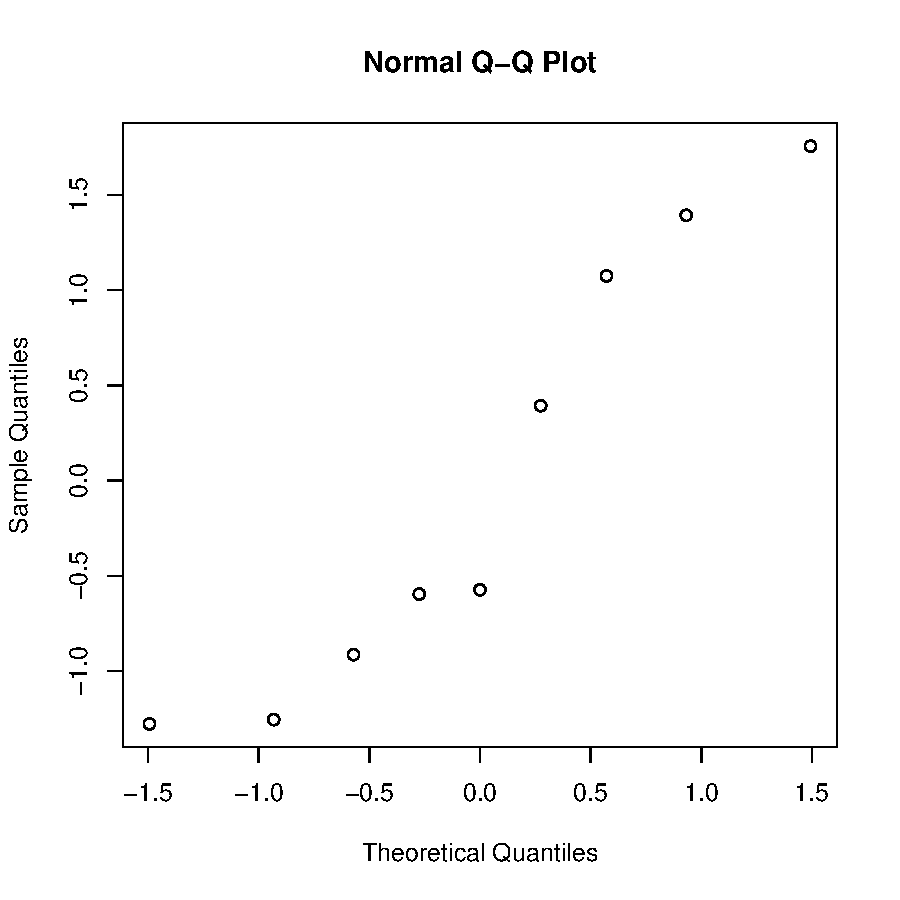
\includegraphics[scale=0.25]{qqtest.pdf}

Para que la normalidad se cumpla los puntos deben estar lo más alineados posible.}
\end{itemize}
\end{frame}
\section{Sumas de cuadrados}
\begin{frame}
\frametitle{Definición de las sumas de cuadrados}

\begin{itemize}
\item<2->{Llamaremos suma de cuadrados de los residuales o del error a
$$SSE=\sum_{i=1}^n(y_i-\hat{y}_i)^2.$$ }
\item<3->{Llamaremos suma de
cuadrados de totales a $$SST =\sum_{i=1}^n(y_i-\overline{y})^2.$$}
\item<4->{Llamaremos suma de cuadrados de la regresión a
$$SSR=\sum_{i=1}^n(\hat{y}_i-\overline{y})^2.$$}
\end{itemize}
\end{frame}

\subsection{Relación entre las sumas de cuadrados}
\begin{frame}
\frametitle{Relación entre las sumas de cuadrados}

\begin{itemize}
\item<2->{En una regresión lineal por el método de mínimos cuadrados se tiene que:
$$SST=SSR+SSE.$$}
\item<3->{La expresión anterior es equivalente a
$$S^2_y=S^2_{\hat{y}}+S^2_e.$$}
\end{itemize}
\end{frame}

\begin{frame}
\frametitle{Ejemplo anterior}
\begin{itemize}
\item<2->{Las sumas de cuadrados son:
$$
\begin{array}{l}
SSE=\sum_{i=1}^n(y_i-\hat{y}_i)^2 =11.06020,\\ SSR=\sum_{i=1}^n(\hat{y}_i-\overline{y})^2 =48.9398,\\
SST =\sum_{i=1}^n(y_i-\overline{y})^2 = 60.
\end{array}
$$
Se puede comprobar que se cumple la igualdad $SST=SSE+SSR$.
}
\end{itemize}
\end{frame}

\section{El coeficiente de determinación $R^2$ y la estimación de la varianza.}
\begin{frame}
\frametitle{El coeficiente de determinación $R^2$ y la estimación de la varianza.}

\begin{itemize}
\item<2->{Se define como $$R^2=\frac{SSR}{SST}.$$}
\item<3->{En el caso de regresión lineal m.c. se cumple que:
$R^2=\frac{S^2_{\hat{y}}}{S^2_y}$, $R^2=1-\frac{SSE}{SST}$, 
$R^2=1-\frac{S^2_e}{S^2_y}$.}
\item<4->{$R^2=r^2_{xy},$ donde $r_{xy}=\frac{s_{xy}}{s_x s_y}$.}
\item<5->{Por lo tanto $R^2$ es la proporción de varianza de la variable $y$
que queda explicada por la regresión lineal.}
\item<6->{Una estimación insesgada de $\sigma^2$ (la varianza del error
$E$) en m.c. es
$$S^2=\frac{SSE}{n-2}.$$}
\end{itemize}
\end{frame}

\begin{frame}
\frametitle{Ejemplo anterior}
\begin{itemize}
\item<2->{El coeficiente $R^2$ valdrá: $R^2 =\frac{48.9398}{60}=0.8157.$ Por tanto, 
se explica el $81.57\%$ de la varianza del crecimiento de la planta.}
\item<3->{Estimación insesgada de la varianza: 
$$S^2 = \frac{SSE}{n-2}=\frac{11.06020}{7}=1.5800.$$}
\end{itemize}
\end{frame}


\section{Intervalos de confianza}
\begin{frame}
\frametitle{Intervalos de confianza}
\begin{itemize}
\item<2->{Suponemos de que los residuos siguen una ley normal.}
\item<3->{Intervalo de confianza al nivel $(1-\alpha)100\%$ para el
parámetro $\beta_1$: ($\mu_{Y/x}=\beta_0+\beta_1 x$)
$$b_1-\frac{t_{n-2,\alpha/2} S}{\sqrt{n S^2_x}}<\beta_1<b_1+\frac{t_{n-2,\alpha/2}S}{\sqrt{
n S^2_x}}$$}
\item<4->{Intervalo de confianza al nivel
$(1-\alpha)100\%$ para el parámetro $\beta_0$: 
$$b_0-\frac{t_{n-2,\alpha/2}S\sqrt{\sum_{i=1}^n x^2_i}}{n
S_{x}}<\beta_0<b_0+\frac{t_{n-2,\alpha/2}S\sqrt{\sum_{i=1}^n
x^2_i}}{n S_{x}}$$}
\end{itemize}
\end{frame}

\begin{frame}
\frametitle{Intervalos de confianza}
\begin{itemize}
\item<2->{Intervalo de confianza al nivel
$(1-\alpha)100\%$ para la respuesta media $\mu_{Y/x_0}$:
$$\hat{y}_0-t_{n-2,\alpha/2}S\sqrt{\frac{1}{n}+\frac{(x_0-\overline{x})^2}{n
S^2_x}}<\mu_{Y/x_0}<$$
$$\hat{y}_0+t_{n-2,\alpha/2}S\sqrt{\frac{1}{n}+\frac{(x_0-\overline{x})^2}{n
S^2_x}}$$}
\item<3->{Intervalo de confianza al nivel
$(1-\alpha)100\%$ para el valor de $y_0$ cuando $x=x_0$:
$$\hat{y}_0-t_{n-2,\alpha/2}S\sqrt{1+\frac{1}{n}+\frac{(x_0-\overline{x})^2}{n
s^2_x}}< y_0 <$$
$$\hat{y}_0+t_{n-2,\alpha/2}S\sqrt{1+\frac{1}{n}+\frac{(x_0-\overline{x})^2}{n
s^2_x}}$$}
\end{itemize}
\end{frame}

\begin{frame}
\frametitle{Ejemplo anterior}
\begin{itemize}
\item<2->{Intervalo de confianza al nivel $95\%$ para la respuesta media $\mu_{Y/x_0}$:
$$
\begin{array}{l}
\hat{y}_0-t_{n-2,\alpha/2}S\sqrt{\frac{1}{n}+\frac{(x_0-\overline{x})^2}{n
s^2_x}}<\mu_{Y/x_0}< \\
\hat{y}_0+t_{n-2,\alpha/2}S\sqrt{\frac{1}{n}+\frac{(x_0-\overline{x})^2}{n
s^2_x}} \\
\hat{y}_0 - t_{7,0.025} \sqrt{\frac{1.58}{9}+\frac{1.58\cdot (x_0 - 6.89)^2}{9\cdot 12.09877}}<\mu_{Y/x_0}< \\
\hat{y}_0 + t_{7,0.025} \sqrt{\frac{1.58}{9} +\frac{1.58\cdot (x_0 - 6.89)^2}{9\cdot 12.09877}} \\
\hat{y}_0 - 2.36\cdot  \sqrt{0.1756 +\frac{(x_0 - 6.89)^2}{68.917}} <\mu_{Y/x_0}< \\
\hat{y}_0 + 2.36\cdot  \sqrt{0.1756 +\frac{(x_0 - 6.89)^2}{68.917}}
\end{array}
$$
Si cogemos $x_0=11$ meses, el intervalo anterior vale: $-0.287<\mu_{Y/x_0}< 2.775.$}
\end{itemize}

\end{frame}

\section{ANOVA}
\begin{frame} 
\frametitle{ANOVA en la recta de regresión lineal}

\uncover<2->{Muy brevemente el Análisis de la Varianza (ANalisys Of VAriance)
consiste en contrastar si la media de una variable en $k$
poblaciones independientes, con distribución normal de igual
varianza, son iguales contra que al menos dos son distintas.
$$\left\{
\begin{array}{rl}
H_0:&\mu_1=\mu_2=\ldots=\mu_k\\
H_1:& \mbox{no todas las medias son iguales}\end{array}\right.$$}


\uncover<3->{En el caso de la regresión lineal, usaremos la técnica anterior para contrastar si las medias de los grupos que conforman las variables son iguales o no (el grupo $k$ está formado por los valores cuya media vale $\mu_{Y/x_k}$). En caso afirmativo, decir que las medias son iguales es equivalente a afirmar que $\beta_1=0$ y, por lo tanto, el modelo de regresión lineal no es bueno.
Por tanto, para que el modelo sea bueno, hemos de rechazar la hipótesis nula en el contraste ANOVA}
\end{frame}

\begin{frame}
\frametitle{ANOVA en la recta de regresión lineal}

\begin{itemize}
\item<2->{Test a realizar:
$$\left\{\begin{array}{rl}H_0:&\beta_1=0\\H_1:&\beta_1\not=0\end{array}\right.$$}

\item<3->{Tabla a calcular:\vskip1cm
\begin{tabular}{|c|c|c|c|c|}\hline
Fuente de & Suma de & g. l. & Cuadrados & \\
variación & cuadrados &  & medios &  $F$\\\hline
Regresión & $SSR$ & $1$ & $SSR$ & $SSR/S^2$ \\
Error & $SSE$ & $n-2$& $S^2=\frac{SSE}{n-2}$ & \\
\hline Total & $SST$ & $n-1$ & & \\\hline\end{tabular}
}
\end{itemize}


\end{frame}

\begin{frame}
\frametitle{ANOVA en la recta de regresión lineal}
\begin{itemize}
\item<2->{Ahora rechazamos la hipótesis nula al nivel de significación $\alpha$ si $f>f_{\alpha,1,n-2}$
donde $f_{\alpha,1,n-2}$ es el valor de una distribución $F$ de
con grados de libertad $1$ y $n-2$.}
\item<3->{Esta prueba, en el caso de regresión lineal simple tiene un efecto
a otra parecida en la que se contrasta con una t de student.}
\end{itemize}

\end{frame}

\begin{frame}
\frametitle{Ejemplo anterior}
\begin{itemize}
\item<2->{Tabla ANOVA:\vskip1cm
\begin{tabular}{|c|c|c|c|c|}\hline
Fuente de & Suma de & g. l. & Cuadrados & \\
variación & cuadrados &  & medios &  $F$\\\hline
Regresión & $48.9398$ & $1$ & $48.9398$ & $30.974$ \\
Error & $11.0602$ & $7$& $S^2=1.5800$ & \\
\hline Total & $60$ & $8$ & & \\\hline\end{tabular}}
\item<3->{Cogemos $\alpha =0.05$. El valor $f_{0.05,1,7}$ vale $5.59$. Como $f=30.974 > 5.59$, rechazamos la hipótesis nula y concluimos que $\beta_1\not=0$. Por tanto, nuestro modelo es adecuado según este análisis.}
\end{itemize}

\end{frame}

\chapter{Regresión lineal múltiple}
%\frame{\partpage}
\section{Introducción}
\begin{frame}
\frametitle{Introducción}
\begin{itemize}
\item<2->{Tenemos $k$ variables independientes $x_1,\ldots, x_k$ y una
variable dependiente $y$.}

\item<3->{Postulamos el modelo de regresión lineal como:
$$\mu_{Y,x_1,\ldots,x_k}= \beta_0+\beta_1 x_1+\ldots\beta_k x_k.$$
Los parámetros $\beta_i$ son desconocidos y se pueden estimar a
partir de una muestra:
$$\{(x_{i1},x_{i2},\ldots,x_{ik},y_i)| i=1,2,\ldots,n\}$$
de la que se exige que $n>k$, es decir el número de observaciones
sea mayor que el número de variables.}
\end{itemize}
\end{frame}

\begin{frame}
\frametitle{Introducción}
\begin{itemize}
\item<2->{El modelo es el siguiente: Consideramos una conjunto de $k$ variables aleatorias $X_{1 },X_{2},\ldots,X_{k}$.
Suponemos que existen variables aleatorias respuestas $Y_1,\ldots,Y_k$ cuya relación con las anteriores es:
$$Y_i=\beta_0+\beta_1 X_{1}+\cdots+\beta_{k} X_k+E_i,$$
donde $E_i$ son variables aleatorias que representan el error aleatorio del modelo asociado a la respuesta $Y_i$.}
\item<3->{El problema es estimar los parámetros $\beta_i$ a
partir de una muestra de datos que representan una muestra aleatoria simple de las variables $X_i$ y de la variable $Y$ de tamaño $n$:
$$\{(x_{i1},x_{i2},\ldots,x_{ik},y_i)| i=1,2,\ldots,n\}.$$
}
\end{itemize}
\end{frame}


\begin{frame}
\frametitle{Introducción}

\begin{itemize}
\item<2->{Llamaremos $y_i$ al valor obtenido de la variable $Y_i$ usando las estimaciones $b_i$ de los parámetros $\beta_i$:
$$y_i=b_0+b_1 x_{i1}+\cdots+b_{k} x_{ik}+e_i\mbox{ para } i=1,2,\ldots,n$$
donde $e_i$ será la estimación de la variable error residual $E_i$ asociado  a la respuesta $Y_i$.}
\item<3->{Llamaremos
$$\hat{y}_i=b_0+b_1 x_{i 1}+\cdots+b_{k} x_{i k}.$$ 
Entonces
$e_i=y_i-\hat{y}_i.$}
\end{itemize}
\end{frame}

\begin{frame}
\frametitle{Introducción}
\begin{itemize}
\item<2->{Definimos los vectores siguientes:
$$
\vect{y}=
\left(
\begin{array}{l}
y_1\\ y_2\\\vdots\\ y_n
\end{array}\right),\  \vect{b}=\left(
\begin{array}{l}
b_0\\ b_1\\\vdots\\b_k
\end{array}\right),\ \vect{\hat{y}}=\left(
\begin{array}{l}
\hat{y}_1\\ \hat{y}_2\\\vdots\\\hat{y}_n
\end{array}\right),\ \vect{e}=\left(
\begin{array}{l}
e_1\\ e_2\\\vdots\\ e_n
\end{array}\right).
$$}
\item<3->{Definimos la matriz siguiente:
$$
\vect{X}=\left(
\begin{array}{lllll}
1&x_{11}&x_{12}&\ldots&x_{1k}\\
1&x_{21}&x_{22}&\ldots&x_{2k}\\
\vdots&\vdots&\vdots&\vdots&\vdots\\
1&x_{n1}&x_{n2}&\ldots&x_{nk}
\end{array}
\right)$$}
\end{itemize}
\end{frame}
\begin{frame}
\frametitle{Introducción}
\begin{itemize}
\item<2->{Podemos escribir el modelo de regresión múltiple matricialmente como:
$$
\begin{array}{rl}
\vect{y}= & \vect{X}\vect{b}+\vect{e},\\
\vect{\hat{y}} = & \vect{X}\vect{b}, \\
\vect{e} = & \vect{y}-\vect{\hat{y}}.
\end{array}$$}
\end{itemize}
\end{frame}

\section{Mínimos cuadrados}
\begin{frame}
\frametitle{Cálculo de los coeficientes $b_i$ usando el método de mínimos cuadrados}
\begin{itemize}
\item<2->{Definimos el error cuadrático $SSE$ como:
$$
\begin{array}{rl}
SSE=&\sum\limits_{i=1}^n
e^2_i=\sum\limits_{i=1}^n (y_i-\hat{y}_i)^2 \\ 
=&\sum\limits_{i=1}^n (y_i-b_0-b_1 x_{i 1}-\cdots -b_{k} x_{ik})^2.
\end{array}$$}
\item<3->{Los estimadores por el método de mínimos cuadrados serán los
valores $b_0,b_1,\ldots, b_k$ que minimicen $SSE$.
}
\item<4->{Para resolver este problema calculamos las derivadas parciales de
SSE respecto a cada $b_i$ para $i=1,2,\ldots,n$ y se obtiene el
un sistema de ecuaciones que recibe el nombre de ecuaciones normales.
}
\end{itemize}
\end{frame}

\begin{frame}
\frametitle{Cálculo de los coeficientes $b_i$ usando el método de mínimos cuadrados}
\uncover<2->{$$
\left.
\begin{array}{rl}
n b_0 +b_1 \sum\limits_{i=1}^n x_{i 1}+\ldots + b_k \sum\limits_{i=1}^n x_{i
k} &=  \sum\limits_{i=1}^n y_i\\ & \\
b_0 \sum\limits_{i=1}^n x_{i 1}+b_1 \sum\limits_{i=1}^n x^2_{i 1}+
b_2\sum\limits_{i=1}^n x_{i 1} x_{i 2}+ \ldots +& \\ &\\ b_k \sum\limits_{i=1}^n x_{i
1}x_{ik} & =  \sum\limits_{i=1}^n x_{i 1}y_i\\
\ldots & \ldots \\
b_0 \sum\limits_{i=1}^n x_{i k}+b_1 \sum\limits_{i=1}^n x_{i k}x_{i 1}+
b_2\sum\limits_{i=1}^n x_{i k} x_{i 2}+\ldots + & \\ &\\  b_k \sum\limits_{i=1}^n x^2_{i
k} & = \sum\limits_{i=1}^n x_{i k}y_i\\\end{array}\right\}
$$}
\end{frame}

\begin{frame}
\frametitle{Cálculo de los coeficientes $b_i$ usando el método de mínimos cuadrados}
\begin{itemize}
\item<2->{El sistema anterior se puede expresar en forma matricial de la forma siguiente: 
$$
\left(\vect{X}^\top\vect{X}\right)\cdot \vect{b}=\vect{X}^\top\cdot \vect{y}.
$$}
\item<3->{La solución buscada del sistema anterior será:
$$
\vect{b}=\left(\vect{X}^\top\vect{X}\right)^{-1}\cdot \left(\vect{X}^\top \vect{y}\right).
$$}
\end{itemize}

\end{frame}
\begin{frame}
\frametitle{Ejemplo}
\begin{itemize}
\item<2->{Se postula que la estatura de un niño recién nacido ($y$)  tiene
una relación con su edad en días $x_1$, su estatura al nacer en
cm. ($x_2$), su peso en Kg. al nacer ($x_3$) y el aumento en tanto por ciento de su peso actual con respecto a su peso al nacer ($x_4$). Se pudo obtener una pequeña muestra con $n=9$
niños cuyos resultados fueron:}
\item<3->{\begin{center}\begin{tabular}{|c|c|c|c|c|}\hline
$y$ & $x_1$ & $x_2$ & $x_3$ & $x_4$\\\hline
57.5&78&48.2&2.75&29.5\\ 52.8&69&45.5&2.15&26.3\\
61.3&77&46.3&4.41&32.2\\ 67&88&49&5.52&36.5\\ 53.5&67&43&3.21&27.2\\
62.7&80&48&4.32&27.7\\ 56.2&74&48&2.31&28.3\\ 68.5&94&53&4.3&30.3\\
69.2&102&58&3.71&28.7\\\hline\end{tabular}\end{center}}
\end{itemize}
\end{frame}
\begin{frame}
\frametitle{Ejemplo}
\begin{itemize}
\item<2->{La matriz $\vect{X}$ es:
$$
\vect{X}=\left(
\begin{array}{lllll}
1&78&48.2&2.75&29.5\\
1&69&45.5&2.15&26.3\\
1&77&46.3&4.41&32.2\\
1&88&49&5.52&36.5\\
1&67&43&3.21&27.2\\
1&80&48&4.32&27.7\\
1&74&48&2.31&28.3\\
1&94&53&4.3&30.3\\
1&102&58&3.71&28.7
\end{array}
\right)
$$}
\end{itemize}
\end{frame}
\begin{frame}
\frametitle{Ejemplo}
\begin{itemize}
\item<2->{El vector $\vect{y}$ es:
$$
\vect{y}=\left(
\begin{array}{l}
57.5\\ 52.8\\ 61.3\\ 67\\ 53.5\\ 62.7\\ 56.2\\ 68.5\\ 69.2
\end{array}
\right)
$$}
\end{itemize}
\end{frame}
\begin{frame}
\frametitle{Ejemplo}
\begin{itemize}
\item<2->{El producto $\vect{X}^\top\vect{X}$ es el siguiente:
$$
\left(
\begin{array}{lllll}
9& 729&   439&  32.68 & 266.7 \\
729& 60123& 35947.2& 2702.41& 21715.3\\
439& 35947.2& 21568.18& 1604.388& 13026.01\\
66.07 & 6108.19 & 3541.008& 128.66&  1948.561\\
266.7& 21715.3&13026.01& 990.27&  7980.83
\end{array}
\right)
$$}
\item<3->{El producto $\vect{X}^\top\vect{y}$ es el siguiente:
$$
\vect{X}^\top\vect{y} = \left(
\begin{array}{l}
548.7\\ 45001\\ 26946.89\\ 2035.52\\ 16348.29
\end{array}
\right)
$$}
\end{itemize}
\end{frame}
\begin{frame}
\frametitle{Ejemplo}
\begin{itemize}
\item<2->{Resolviendo el sistema $(\vect{X}^\top\vect{X})\cdot \vect{b}=\vect{X}^\top \vect{y}$ obtenemos como solución:
$$
\vect{b}=\left(
\begin{array}{l}
7.1475 \\ 0.1001 \\ 0.7264 \\ 3.0758\\ -0.03
\end{array}
\right)
$$}
\item<3->{La recta de regresión estimada es :
$$\hat{y}=7.1475 +   0.1001 x_1+0.7264 x_2 +3.0758 x_3-0.03 x_4.$$}
\end{itemize}
\end{frame}
\section{Propiedades}
\begin{frame}
\frametitle{Propiedades de la recta de regresión}
\begin{itemize}
\item<2->{La recta de regresión ajustada pasa por el vector de
medias. O sea, si llamamos $\overline{x}_j=\frac{\sum\limits_{i=1}^n x_{ij}}{n},$ para $i=1,\ldots,k$, $\overline{y}=\frac{\sum\limits_{i=1}^n y_i}{n}$, se verifica que:
$$
\overline{y}=b_0 + b_1\overline{x}_1+\cdots +b_k \overline{x}_k.
$$}
\item<3->{La suma de los errores $e_i$ es $0$: $\sum\limits_{i=1}^n
e_i=0$ y por lo tanto su media también: $\overline{e}=0$.}
\item<4->{La media de los valores estimados coincide con la media de los valores de la muestra: $\overline{\hat{y}}=\overline{y}$.}
\end{itemize}
\end{frame}
\begin{frame}
\frametitle{Ejemplo}
\begin{itemize}
\item<2->{Veamos que la recta de regresión pasa por el vector de medias. Éste vale:
$$
\overline{x}_0 = 1,\ \overline{x}_1=81,\ \overline{x}_2 =48.778,\ \overline{x}_3=3.631,\ \overline{x}_4 = 29.633.
$$
La media del vector $\vect{y}$ vale: $\overline{y}=60.967$.

Se cumple:
$$
\begin{array}{rl}
60.967 \approx  & 7.1475 +  0.1001\cdot 81 +0.7264\cdot 48.778 \\ & +3.0758\cdot 3.6311-0.03\cdot 29.633.
\end{array}
$$
}

\end{itemize}
\end{frame}

\begin{frame}
\frametitle{Ejemplo}
\begin{itemize}
\item<2->{Veamos que la media de los errores es nula.
Los valores de los vectores $\vect{\hat{y}}$ y $\vect{e}$ son:
$$
\vect{\hat{y}}=\vect{X}\cdot b =  \left(\begin{array}{l}
 57.541 \\  52.929 \\  61.085 \\ 67.432 \\ 54.146 \\  62.479 \\ 55.678  \\   67.372 \\ 70.039      \end{array}\right),\ \vect{e}=\vect{y}-\vect{\hat{y}}=\left(\begin{array}{l}
    -0.0405\\ -0.1290\\ 0.2150\\ -0.4324 \\ -0.6461 \\ 0.2214 \\ 0.5225 \\ 
 1.1277\\ -0.8385 \end{array}\right)
$$}
\item<3->{Puede comprobarse que la media del vector $\vect{e}$ es $0$ y que $\overline{\hat{y}}=\overline{y}=60.967$.}
\end{itemize}
\end{frame}


\section{Sumas de cuadrados}
\begin{frame}
\frametitle{Sumas de cuadrados en la regresión}
\begin{itemize}
\item<2->{Llamaremos suma de cuadrados de los residuales o del error a
$$SSE=\sum_{i=1}^n (y_i-\hat{y}_i)^2.$$}
\item<3->{Llamaremos suma de cuadrados de totales a 
$$SST=\sum_{i=1}^n (y_i-\overline{y})^2.$$}
\item<4->{Llamaremos suma de
cuadrados de la regresión a
$$SSR=\sum_{i=1}^n(\hat{y}_i-\overline{y})^2.$$}
\item<5->{Se verifica:
$$SST=SSR+SSE,$$
o equivalentemente:
$$S^2_y=S^2_{\hat{y}}+S^2_e.$$}
\end{itemize}
\end{frame}

\begin{frame}
\frametitle{Ejemplo}
\begin{itemize}
\item<2->{La suma de cuadrados del error vale en el ejemplo anterior:
$$
SSE =(57.5-57.5405)^2+\cdots +(69.2-70.0385)^2 = 2.9656.
$$}
\item<3->{La suma de cuadrados totales vale:
$$
SST=(57.5-60.967)^2+\cdots +(69.2-60.967)^2 = 321.24.
$$}
\item<4->{La suma de cuadrados de la regresión es:
$$
\begin{array}{rl}
SSR= & (57.5405-60.967)^2 +\cdots +(70.0385-60.967)^2 \\ 
= & 318.274.
\end{array}
$$}
\item<5->{Puede observarse que se cumple: 
$$
SST=SSE+SSR,\quad 321.24 = 2.9656 + 318.274.
$$}
\end{itemize}
\end{frame}


\section{Coeficiente de determinación}
\begin{frame}
\frametitle{Definición del coeficiente de determinación}
\begin{itemize}
\item<2->{Definimos el coeficiente de determinación como
$$R^2=\frac{SSR}{SST}=1-\frac{SSE}{SST},$$
o también
$$R^2=\frac{S^2_{\hat{y} }}{S^2_y}=1-\frac{S^2_e}{S^2_y}.$$
$R^2$  se interpreta como la proporción de varianza de la variable
$y$ que es explicada por el modelo de regresión múltiple.
}
\item<3->{Definimos el coeficiente de determinación ajustado como:
$$R^2a=R^2-\frac{k(1-R^2)}{n-k-1}.$$}
\item<4->{Definimos el coeficiente de correlación múltiple $r$ de la variable $y$ respecto de las variables $x_1,\ldots, x_k$ como $r=\sqrt{R^2}$.}
\end{itemize}
\end{frame}

\begin{frame}
\frametitle{Ejemplo}
\begin{itemize}
\item<2->{El coeficiente de determinación vale en nuestro ejemplo:
$$
R^2 = \frac{318.274}{321.24} \approx 0.9908.
$$}
\item<3->{El coeficiente de determinación ajustado vale:
$$
R^2a = 0.9908 -\frac{4\cdot (1-0.9908)}{9-4-1} = 0.9815.
$$}
\item<4->{El coeficiente de correlación múltiple $r$ de la variable $y$ respecto de las variables $x_1,\  x_2,\ x_3,\ x_4$ vale: $r=\sqrt{0.9908}=0.9954.$}
\end{itemize}
\end{frame}
\section{Consideraciones sobre el modelo}
\begin{frame}
\frametitle{Consideraciones sobre el modelos de regresión múltiple}
\begin{itemize}
\item<2->{Suponemos que las variables aleatorias error $E_i$ son
independientes e idénticamente distribuidas  según una normal de
media $0$ y varianza $\sigma^2$.}
\item<3->{Bajo el supuesto anterior,
los estimadores $b_0,\ldots, b_k$ de
$\beta_0,\ldots,\beta_k$ son insesgados. O sea, $E(b_i)=\beta_i,\ i=0,\ldots, k$.}
\item<4->{La matriz $(X^\top X)^{-1} \sigma^2$ es la matriz de covarianzas de
$\beta_0,\ldots,\beta_k$.}
\item<5->{Un estimador insesgado de
$\sigma^2$ es $$S^2=\frac{SSE}{n-k-1}.$$}
\end{itemize}
\end{frame}
\begin{frame}
\frametitle{Ejemplo}
\begin{itemize}
\item<2->{Una estimación de la varianza $\sigma^2$ será:
$$
S^2 = \frac{2.9656}{9-4-1}=0.7414.
$$}
\item<3->{Una estimación de la matriz de covarianzas de $\beta_0,\ldots, \beta_4$: $(X^\top X)^{-1} S^2 = $
$$
\left(
\begin{array}{lllll}
270.919 & 5.325 &  -12.521 &  -13.743 &  -1.4 \\
5.325 & 0.115 & -0.266 & -0.326 & -0.0176 \\
-12.521 &  -0.266 & 0.618 &  0.742 & 0.0416 \\
-13.743 &  -0.326 &  0.742 &  1.122 &  -0.00598 \\
-1.4 & -0.0176 & 0.0416 &  -0.00598 &  0.0277
\end{array}
\right)
$$}
\end{itemize}
\end{frame}
\section{ANOVA}
\begin{frame}
\frametitle{ANOVA en regresión lineal múltiple}
\begin{itemize}
\item<2->{El contraste ANOVA en la regresión lineal múltiple nos permite contrastar la adecuación del modelo. Se trata de contrastar: 
$$\left\{\begin{array}{rl} H_0:& \beta_1=\beta_2=\cdots=\beta_k=0 \\
H_1: & \mbox{hay alguna }\beta_i\not= 0 \end{array}\right.$$
}
\item<3->{Si aceptamos $H_0$ estamos diciendo que la estimación dada por la
regresión es constante. Por tanto el modelo no sería adecuado.}
\item<4->{En la tabla siguiente aparece los pasos necesarios para realizar el contraste. Como puede observarse, se usa como estadístico de contraste el cociente $\frac{MSR}{MSE}$ que, suponiendo normalidad, sigue una distribución $F$ de Snédecor de $k,n-k-1$ grados de libertat:
}
\end{itemize}
\end{frame}
\begin{frame}
\frametitle{ANOVA en regresión lineal múltiple}
\uncover<2->{\begin{tabular}{|c|c|c|c|c|}\hline
F.V. & S.C. & g.l. & C.M. & $f$\\\hline
Regresión & $SSR$ & $k$ & $MSR=\frac{SSR}{k}$ & $f=\frac{MSR}{MSE}$ \\ &&&&\\
Error & $SSE$ & $n-k-1$& $MSE=\frac{SSE}{n-k-1}$ & \\
\hline Total & $SST$ & $n-1$ & & \\\hline\end{tabular} 
\begin{description}
\item F.V.: Fuente de variación.
\item S.C.: Suma de cuadrados.
\item g.l.: grados de libertad.
\item C.M.: Cuadrados medios.
\end{description}
}
\uncover<3->{Rechazaremos la hipótesis nula  $H_0: \beta_1=\ldots=\beta_k =0$ al
nivel de significación $\alpha$ si $f>f_{\alpha,k,n-k-1}$
donde $f_{\alpha,k,n-k-1}$ es el valor crítico de una distribución
$F$ de con grados de libertad $k$ y $n-k-1$.}
\end{frame}
\begin{frame}
\frametitle{Ejemplo}
\begin{itemize}
\item<2->{La tabla ANOVA es en nuestro ejemplo:
\begin{center}\begin{tabular}{|c|c|c|c|c|}\hline
F.V. & S.C. & g.l. & C.M. & $f$\\\hline
Regresión & $318.274$ & $4$ & $MSR=79.569$ & $f=107.323$ \\ &&&&\\
Error & $2.9656$ & $4$& $MSE=0.7414$ & \\
\hline Total & $321.24$ & $8$ & & \\\hline\end{tabular}\end{center}}
\item<3->{Cogiendo $\alpha =0.05$, el valor crítico $f_{0.05,4,4}$ vale $6.388.$ Como $f=107.323 > f_{0.05,4,4}=6.388$, rechazamos la hipótesis nula y concluimos que el modelo es adecuado según este análisis.}
\end{itemize}
\end{frame}
\begin{frame}
\frametitle{ANOVA en regresión lineal múltiple}
\begin{itemize}
\item<2->{El modelo de regresión lineal con este conjunto de $x$
puede no ser el único que se puede utilizar. Es posible que con
algunas transformaciones de las $x$ mejore el valor de $f$.}
\item<3->{El modelo podría ser más eficaz si se incluyen otras variables o
podría continuar siendo casi igual de eficaz si se eliminan
algunas (principio de parsimonia).}
\end{itemize}
\end{frame}
\section{Intervalos de confianza}
\begin{frame}
\frametitle{Intervalos de confianza}
\begin{itemize}
\item<2->{Un intervalo de confianza al nivel $(1-\alpha) 100\%$ para la
respuesta media $\mu_{Y/x_{10},x_{20},\ldots,x_{k0}}$ es
$$\hat{y}_0 -t_{\alpha/2,n-k-1} S\sqrt{x^\top_0 (X^\top X)^{-1}
x_0}<$$
$$\mu_{Y/x_{10},x_{20},\ldots,x_{k0}} <\hat{y}_0
+t_{\alpha/2,n-k-1} S\sqrt{x^\top_0 (X^\top X)^{-1} x_0}$$
donde $t_{\alpha/2,n-k-1}$ es el valor crítico de una $t$ de
student con $n-k-1$ grados de libertad, 
$x_0=\left(1,
x_{10},x_{20},\ldots ,x_{k0}\right)^\top$ y $\hat{y}_0 = b_0 + b_1 x_{10} + \cdots +b_k x_{k0}.$}
\item<3->{La cantidad $S\sqrt{x^\top_0 (X^\top X)^{-1} x_0}$ recibe el nombre de
error estándar de predicción.
}
\end{itemize}
\end{frame}
\begin{frame}
\frametitle{Ejemplo}
\begin{itemize}
\item<2->{Para $\alpha =0.05$, hallemos un intervalo de confianza para la respuesta media $\mu_{Y/x_{10},x_{20},x_{30},x_{40}}$, para $x_{10} =69,\ x_{20} = 45.5,\ x_{30} = 2.15,\  x_{40} = 26.3$.}
\item<3->{El valor crítico $t_{0.025,4}$ vale $2.776$. El valor $\hat{y}_0$ valdrá:
$$
\begin{array}{rl}
\hat{y}_0 = & b_0 +\sum_{i=1}^4 b_i x_{i0} \\
= & 7.1475+0.1001\cdot 69 +0.7264\cdot 45.5+3.0758\cdot 2.15 \\ & -0.03\cdot 26.3 
=  52.929.
\end{array}
$$}
\item<4->{
El valor de $x^\top_0 (X^\top X)^{-1} x_0$ es:
$$
(1,69,45.5,2.15,26.3)\cdot (X^\top X)^{-1}\cdot \left(\begin{array}{l}
1\\ 69 \\ 45.5\\ 2.15 \\ 26.3\end{array}\right) = 0.3615.
$$}
\end{itemize}
\end{frame}
\begin{frame}
\frametitle{Ejemplo}
\uncover<2->{El intervalo de confianza será:
$$
\begin{array}{l}
52.929-2.776\sqrt{0.7414\cdot 0.3615}<\mu_{Y/x_{10},x_{20},x_{30},x_{40}} \\
< 52.929+2.776\cdot\sqrt{0.7414\cdot 0.3615} = \\
51.492 <\mu_{Y/x_{10},x_{20},x_{30},x_{40}} < 54.366.
\end{array}
$$
}
\end{frame}
\begin{frame}
\frametitle{Intervalos de confianza}
\begin{itemize}
\item<2->{Un intervalo de confianza al nivel $(1-\alpha) 100\%$ para
una predicción individual $y_0$ para los valores de la variables
dependientes $x_{10},x_{20},\ldots,x_{k0}$ es
$$ \hat{y}_0 -t_{\alpha/2,n-k-1} S\sqrt{1+x^\top_0 (X^\top X)^{-1} x_0}<y_0
<$$
$$\hat{y}_0 +t_{\alpha/2,n-k-1} S\sqrt{1+x^\top_0 (X^\top X)^{-1}
x_0},$$
donde $t_{\alpha/2,n-k-1}$ es el valor crítico de una $t$ de
student con $n-k-1$ grados de libertad, y
$x_0=\left(1,x_{10},x_{20},\ldots,x_{k0}\right)^\top.$}
\end{itemize}
\end{frame}
\begin{frame}
\frametitle{Intervalos de confianza}
\begin{itemize}
\item<2->{Un intervalo de confianza al nivel $(1-\alpha) 100\%$ para el parámetro $\beta_k$ es:
$$
b_k -t_{\alpha/2,n-k-1} s_{\beta_k} < \beta_k < b_k + t_{\alpha/2,n-k-1} s_{\beta_k},
$$
donde $s_{\beta_k}$ es la raiz cuadrada del elemento $k$-ésimo de la diagonal de la matriz $(X^\top X)^{-1} S^2$:
$s_{\beta_k} =\sqrt{\left((X^\top X)^{-1} S^2 \right)_{kk}}$.}
\end{itemize}
\end{frame}
\begin{frame}
\frametitle{Ejemplo}
\begin{itemize}
\item<2->{Para $\alpha =0.05$, hallemos un intervalo de confianza para el parámetro $\beta_2$.}
\item<3->{El valor crítico $t_{0.025,4}$ vale $2.776$. Los valores de la diagonal de la matriz $(X^\top X)^{-1} S^2$ son:
$$
270.919,\quad 0.1154,\quad 0.6176,\quad 1.1219,\quad 0.02775.
$$
El valor que nos interesa es para el parámetro $\beta_2$: $0.726$.}
\item<4->{El intervalo será:
$$
\begin{array}{rl}
0.726-2.776\cdot \sqrt{0.6176}<  & \beta_2  \\ <  0.726+2.776\cdot \sqrt{0.6176} , &\\
-1.4556 < & \beta_2 < 2.908.
\end{array}
$$}
\end{itemize}
\end{frame}

\section{Selección del modelo. Colinealidad}
\begin{frame}
\frametitle{El problema de la selección del modelo. Colinealidad}
\begin{itemize}
\item<2->{Dado un problema regresión lineal múltiple podemos  ajustar
todos los submodelos lineales posibles
$$
\begin{array}{rl}
Y=&\beta_0+ \beta_1 x_1,\\
Y=&\beta_0+ \beta_1 x_1+\beta_2 x_2,\\
&\ldots\\
Y=&\beta_0+ \beta_1 x_1+\cdots +\beta_k x_k,
\end{array}
$$
ya que es posible que entre variables $x_i$ exista una fuerte
relación lineal y entonces \emph{sobren del modelo}. Este problema
recibe el nombre de colinealidad.}
\item<3->{Existen también otro tipo de problemas que se pueden resolver usando la técnica de la regresión lineal múltiple. Véase como ejemplo el problema de la regresión polinomial:
$$Y=\beta_0+ \beta_1 x+\beta_2 x^2+\cdots +\beta_k x^k.$$
}
\end{itemize}
\end{frame}
\begin{frame}
\frametitle{El problema de la selección del modelo. Colinealidad}
\uncover<2->{Una solución para ver qué modelo lineal es el más simple y
adecuado es  recurrir a los llamados métodos secuenciales de
selección del modelo lineal, como son los siguientes:
\begin{itemize}
\item Regresión paso paso (Stepwise). 
\item Selección hacia adelante(Forward).
\item Selección hacia atrás (Backward).
\end{itemize}
}
\end{frame}

